
\section{Introdução}




\noindent \begin{minipage}[c]{0.6\textwidth}
  \vspace {1cm}
  \begin{description}
    \item [Banana] Exemplo de mini página com figura e seus respectivos rotulos, para que sejam referenciados ao decorrer do texto.
    \item [Maça] Veja que a Figura \ref{fig:place}, está reservando um espaço para adição de figuras, e o mesmo já esta referenciando seu autor e sua nomeclatura com o indice automatico.
  \end{description}

\end{minipage}
\begin{minipage}[c]{0.4\textwidth}
  \captionof{figure}{Placeholder.}
  
\includegraphics[width=\textwidth]{figure/placeholder.jpg}
  \label{fig:place}
  {\fontsize{10pt}{\baselineskip}\selectfont
    Fonte: \citeonline{linux:2023}}
\end{minipage}


\section{Desenvolvimento}




\lstinputlisting[language=c, caption={código externo}, label={cod:externo}]{main.c} %Busca os codigos na pasta /cod




\begin{figure}[H] %Figuras da aula pratica 1.1
  \center
  \subfigure[ Algoritmo.\label{fig:pri2}]{
\includegraphics[scale=0.4]{figure/placeholder.jpg}}
  \subfigure[Comportamento.\label{fig:seg2}]{
\includegraphics[scale=.4]{figure/placeholder.jpg}}
  \caption{Resultado da atividade prática 1.2, \cite{oliveira_SO2009}}\label{fig:ap1_cod_vigual1}
\end{figure}

%%%%%%%%%%%%%%%%%%%%%%%%%%%%%%%%%%%%%%%%%%%%%%%%%%%%%%%%%%


Para referenciar utilize \cite{ninguem2022curioso}. Também pode ser citado integrada ao texto, de acordo com \citeonline{alguem2022nada}.


\begin{figure}[H]
\centering
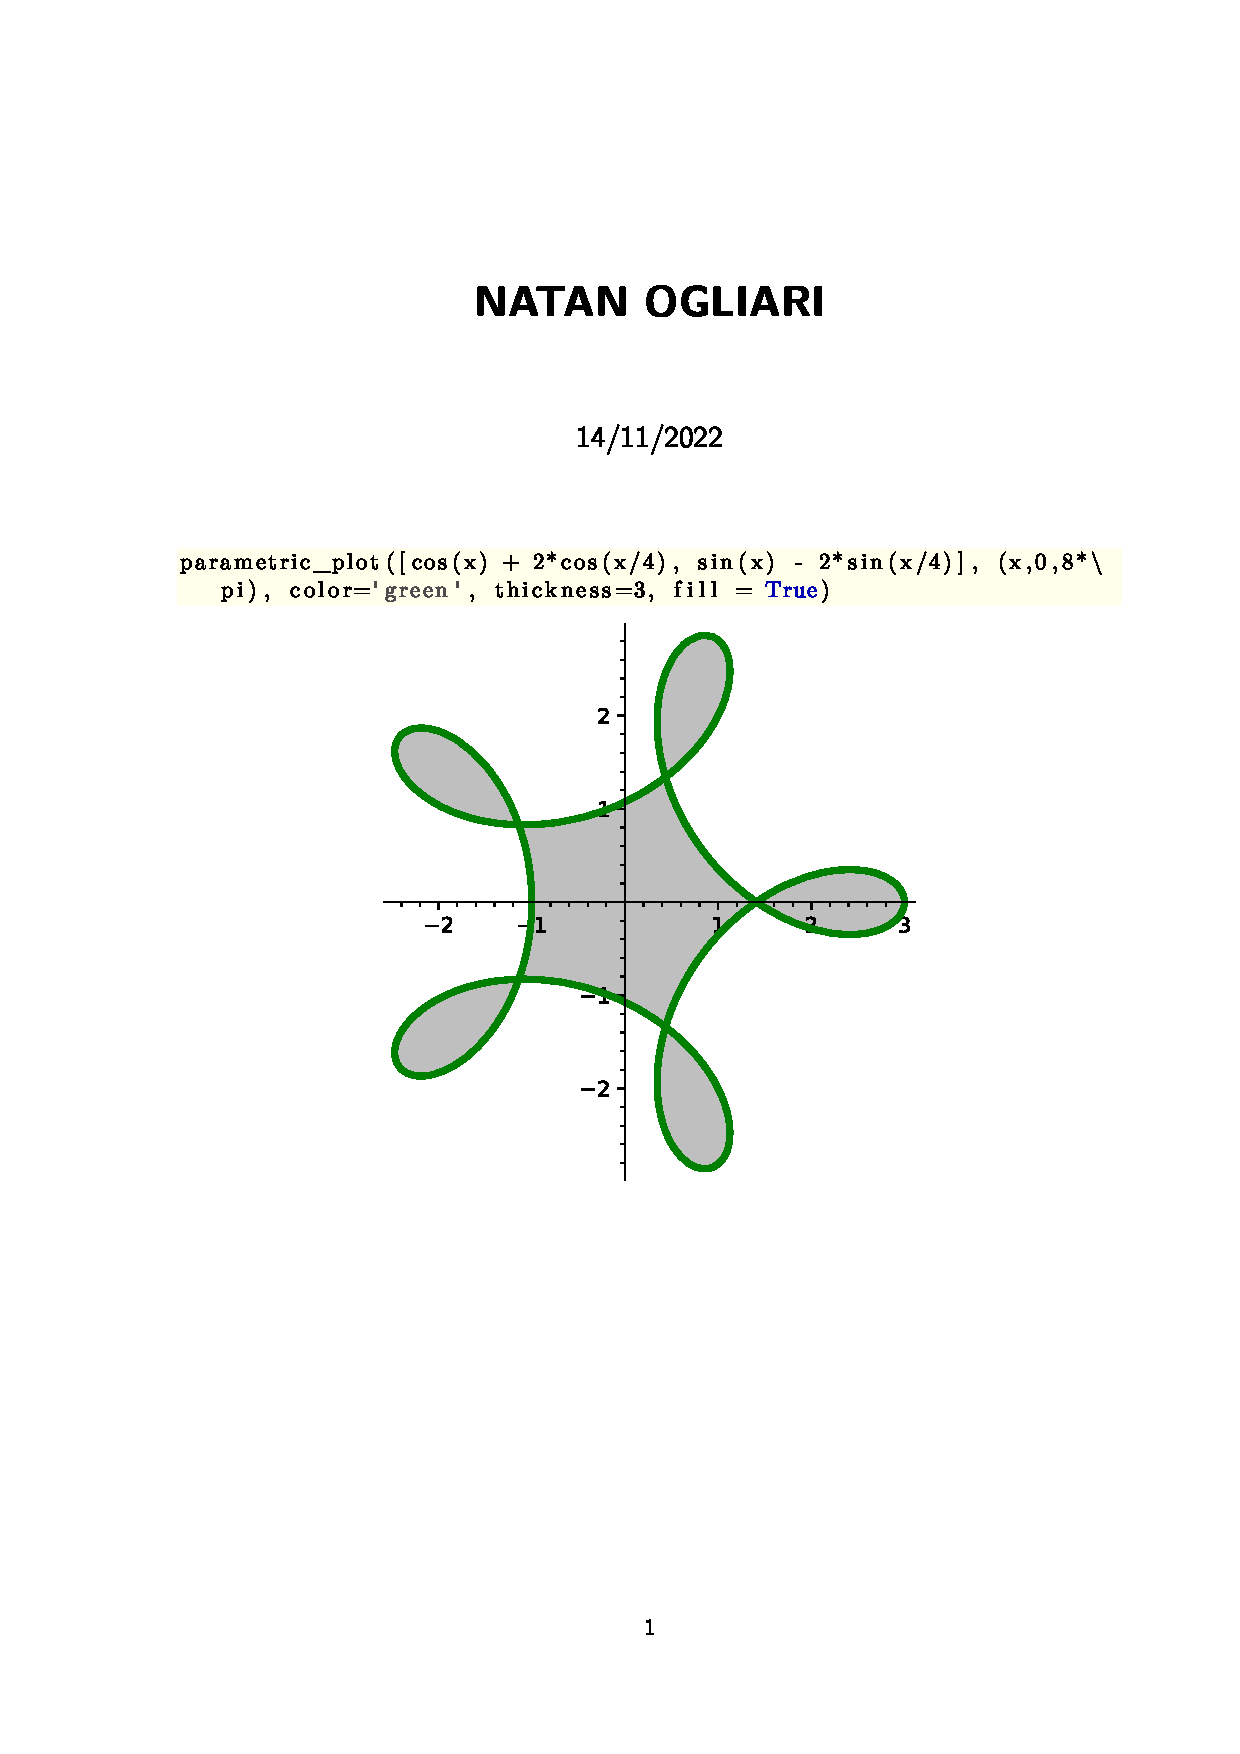
\includegraphics[width=1\textwidth]{figure/Welcome to CoCalc.pdf}
\caption{Exemplo de uma imagem bem massa aqui, o autor}
\label{fig:imagem_massa}
\end{figure}

\par Estou usando \href {https://cocalc.com/} {CoCal}

E para referenciar a figura \ref{fig:imagem_massa} utilize dessa forma.


\begin{enumerate}[label=\Roman{*}, ref=(\roman{*})]
  \item fsfsdf
  \item kugfhiuh
\end{enumerate}

\begin{asparaenum}
\item Anterior ... \cite{ninguem2022curioso}
\item Próximo ... \label{pl1}
\end{asparaenum}



\section{Conclusões}

\begin{algorithm}
\DontPrintSemicolon
\KwData{Ponteiros randomicos.} \Comment{Testando meu comentario} \\
\KwResult{Ordenação de vetores, e concatenação de vetores.}

\Begin{ \Comment{Inicio do meu algoritimo.} \\
$V \longleftarrow X$\;
$S \longleftarrow \emptyset$\;
\For{$x\in X$}{
  $NbSuccInS(x) \longleftarrow 0$\;
  $NbPredInMin(x) \longleftarrow 0$\;
  $NbPredNotInMin(x) \longleftarrow |ImPred(x)|$\;
}
\For{$x \in X$}{
  \If{$ponteiroValido() = 1$ {\bf and} $filaVazia() = 1$}{
    $SOMA4()$}
    }
\nl\While{$S \neq \emptyset$}{\label{InRes1}
\nlset{REM} remove $x$ from the list of $T$ of maximal index\;\label{InResR}
\lnl{InRes2}\While{$|S \cap ImSucc(x)| \neq |S|$}{
\For{$ y \in S-ImSucc(x)$}{
\{ remove from $V$ all the arcs $zy$ : \}\;
\For{$z \in ImPred(y) \cap Min$}{
remove the arc $zy$ from $V$\;
$NbSuccInS(z) \longleftarrow NbSuccInS(z) - 1$\;
move $z$ in $T$ to the list preceding its present list\;
\{i.e. If $z \in T[k]$, move $z$ from $T[k]$ to
$T[k-1]$\}\;
}
$NbPredInMin(y) \longleftarrow 0$\;
$NbPredNotInMin(y) \longleftarrow 0$\;
$S \longleftarrow S - \{y\}$\;
$AppendToMin(y)$\;
}
}
$RemoveFromMin(x)$\;
}
}
\caption{Exemplo de algoritimo}
\end{algorithm}


  %$X \xLongleftarrow[\text{NATAN}]{\text{OGLIARI}} Y $ %COM TEXTO
	% $\uparrow$ %Seta para Cima
	%$\overleftarrow{NATAN}$
